\section{Dodatek}

\subsection{Przebieg poświęcenia wody}
\label{sec:woda}
\begin{enumerate}
      \item \textit{Dominus Vobiscum} i Oracja 0. (przed wejściem)
            \smallfont{(złożone ręce)}
      \item \textit{Dominus Vobiscum} i Oracja 1. \smallfont{(złożone ręce)}
      \item Prefacja do słów \textit{Sumat unigeniti tui gratiam de Spiritu
                  Sancto}
      \item Celebrans kreśli znak krzyża
            \textcolor{red}{\raisebox{-1mm}{\scalebox{1.5}{\ding{64}}}} na
            wodzie
      \item Wyciera ręce
      \item Kontynuuje modlitwę
      \item Na \textit{Sit haec} kładzie rękę na powierzchni wody
      \item Wyciera rękę
      \item Kreśli znaki krzyża
            \textcolor{red}{\raisebox{-1mm}{\scalebox{1.5}{\ding{64}}}}
            nad wodą na słowa \textit{Per Deum vivum \dots}
            \vspace*{-11pt}
      \item Wylewa wodę na cztery strony świata po słowach \textit{... super te
                  ferebatur} ~~~
            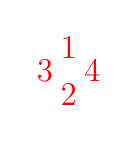
\begin{tikzpicture}[scale=0.3, baseline=-1mm, thick]
                  \draw[color=red] (10mm,0) node {\large 4};
                  \draw[color=red] (-10mm,0) node {\large 3};
                  \draw[color=red] (0,10mm) node {\large 1};
                  \draw[color=red] (0,-10mm) node {\large 2};
            \end{tikzpicture}
            \vspace*{-7pt}
      \item Kreśli znak krzyża nad wodą na \textit{Benedico te}
      \item Po zmianie głosu na \textit{recto tono} na słowa \textit{tu benignus
                  aspira} trzy razy dmucha do wody na kształt krzyża
      \item W tym czasie ceremoniarz podaje Paschał
      \item Na słowa \textit{Descendad in hanc} trzy razy wkłada Paschał do wody
            i śpiewa \footnote{Wkłada Paschał coraz głębiej}
      \item \ii~ trzy razy dmucha do wody w kształcie litery
            \textcolor{red}{\raisebox{-1mm}{\Large ${\Psi}$}} i kontynuuje
            \textit{Totamque ... effectu}
      \item Wyciągamy Paschał z wody i kończymy święcenie wody (\textit{... per
                  ignem.})
      \item Po wyjęciu paschału nabiera się wody do pokropienia
      \item Następnie \cc1 przynosi do chrzcielnicy tackę z olejami świętymi i
            wręcza \ii~ (z pocałunkiem) odpowiednie ampułki. \ii, wypowiadając
            słowa przepisane w księdze po kolei:
            \begin{itemize}
                  \item wlewa olej katechumenów
                  \item wlewa krzyżmo
                  \item wlewa oba
            \end{itemize}
      \item Następnie miesza wodę ręką lub przy pomocy łyżeczki
      \item Później myje i wyciera ręce \footnote{W razie potrzeby wykorzystuje
                  sól, watę i miękisz chleba, które później należy spalić. Wodę
                  z tej ablucji wlewa
                  się do sacrarium.}
\end{enumerate}

\subsection{Bierzmowanie}
\label{sec:bierz}
\begin{itemize}
      \item księgę z modlitwami trzyma \cc1, a \cc2 podtrzymuje kapę jeśli
            trzeba; \aa1 i \aa2 stoją z boku przy kredencji
      \item \ii~ odmawia modlitwę zwracając się do kandydatów \textit{Spiritus
                  Sanctus superveniat\dots}
      \item \ii~ czyni znak Krzyża Świetego mówiąc \textit{Adjutorium
                  nostrum...} a następnie kontynuowany jest krótki dialog
      \item \ii~ wyciąga ręce nad przystępującymi do bierzmowania i mówi
            \textit{Oremus. Omnipotens sempiterne Deus,...}
      \item przystępujący do sakramentu klęka przed \ii. Świadek kładzie rękę na
            prawym ramieniu bierzmowanego.
      \item \aa1 podchodzi do \ii~ z Krzyżmem Świętem
      \item \ii~ kładzie prawą rękę na głowie bierzmowanego i palcem umoczonym w
            Krzyżmie Świętym robi znak krzyż a na czole, mówiąc \textit{Signo te
                  signo...}
      \item \ii~ uderza lekko w policzek bierzmowanego, mówiąc \textit{Pax tecum}
      \item kandydat wraca na swoje wcześniejsze miejsce i stoi
      \item \aa1 odbiera Krzyżmo, a \aa2 podchodzi z czymś do wytarcia palców
            \footnote{najpewniej wata}; później wracają do kredencji
      \item gdy \ii~ namaści wszystkich kandydatów, śpiewa się antyfonę
            \textit{Confirma hoc, Deus\dots}
      \item powtarza się antyfonę, a następnie \ii~ zwrócony do ołtarza śpiewa
            \textit{Ostende nobis, Domine,...}, a następnie \textit{Oremus.
                  Deus, qui Apostolis tuis\dots}
      \item \ii~ mówi \textit{Ecce sic benedicetur omnis homo, qui timet Dominum}
      \item na końcu \ii~ błogosławi bierzmowanych
            \textit{Bene} + \textit{dicat vos Dominus ex Sion...}
\end{itemize}

\color{red}

\section{Uwagi}
\begin{itemize}
      \item można zrobić jakieś święcenie ognia przed proroctwami tak aby ludzie
            oświetlali kościół i mieć jakąś namiastkę Wigilii Paschalnej
      \item na poświęcenie wody ludzie \textbf{muszą mieć zapalne świece}
      \item zapytać księdza czy będzie aspersja (czy to humanitarne?)
      \item ziomek do chrztu musi siedzieć za kratą aż do ochrzczenia -- trzeba
            mu przygotować jakieś krzesło i klęcznik
      \item na chrzest dorosłego ksiądz ubiera kapę (patrz Nowowiejski)
\end{itemize}